%%%%%%%%%%%%%%%%%%%%%%%%%%%%%%%%%%%%%%%%%
% University/School Laboratory Report
% LaTeX Template
% Version 3.0 (4/2/13)
%
% This template has been downloaded from:
% http://www.LaTeXTemplates.com
%
% Original author:
% Linux and Unix Users Group at Virginia Tech Wiki 
% (https://vtluug.org/wiki/Example_LaTeX_chem_lab_report)
%
% License:
% CC BY-NC-SA 3.0 (http://creativecommons.org/licenses/by-nc-sa/3.0/)
%
%%%%%%%%%%%%%%%%%%%%%%%%%%%%%%%%%%%%%%%%%

%----------------------------------------------------------------------------------------
%	PACKAGES AND DOCUMENT CONFIGURATIONS
%----------------------------------------------------------------------------------------

\documentclass{article}

\usepackage[version=3]{mhchem} % Package for chemical equation typesetting
\usepackage{siunitx} % Provides the \SI{}{} command for typesetting SI units

\usepackage{graphicx}
\usepackage{caption}
\usepackage{subcaption}
\usepackage{cancel}

\usepackage{float}

\usepackage[T1]{fontenc} % allow small bold caps

\usepackage{listings}
\usepackage{color}

\definecolor{dkgreen}{rgb}{0,0.6,0}
\definecolor{gray}{rgb}{0.5,0.5,0.5}
\definecolor{mauve}{rgb}{0.58,0,0.82}

\lstset{frame=tb,
  language=Matlab,
  aboveskip=2mm,
  belowskip=2mm,
  showstringspaces=false,
  columns=flexible,
  basicstyle={\small\ttfamily},
  numbers=none,
  numberstyle=\tiny\color{gray},
  keywordstyle=\color{blue},
  commentstyle=\color{dkgreen},
  stringstyle=\color{mauve},
  breaklines=true,
  breakatwhitespace=true
  tabsize=2
}

\setlength\parindent{0pt} % Removes all indentation from paragraphs

\renewcommand{\labelenumi}{\alph{enumi}.} % Make numbering in the enumerate environment by letter rather than number (e.g. section 6)

\usepackage[margin=1in]{geometry}

\usepackage{amssymb}


%\usepackage{times} % Uncomment to use the Times New Roman font

%----------------------------------------------------------------------------------------
%	Title
%----------------------------------------------------------------------------------------

\begin{document}
\pagenumbering{gobble}

\title{6.s02: EECS II - From A Medical Perspective}
\author{
  Ryan Lacey <rlacey@mit.edu>\\
  \footnotesize \texttt{Collaborator(s): Jorge Perez}
}
        
\maketitle
        


\begin{enumerate}
\item[1.]
	\begin{enumerate}
	\item[(a)]
		Average heart rate: 87.7 bpm\\
		Standard deviation of RR interval: 0.0021\\
\begin{lstlisting}   
function [ times, rrt ] = ecg2rr( ecg, minheight, mindistance )
    t = linspace(0, 30+(5/60), length(ecg));
    [pks, locs] = findpeaks(ecg, 'MINPEAKHEIGHT', minheight, 'MINPEAKDISTANCE', mindistance);
    times = diff(t(locs));
    rrt = t(locs(2:end));
end

sum(times.^-1)/length(times) %bpm
std(rrt) %std
\end{lstlisting}

\bigskip

	\item[(b)]
		K=2\\
		Centroids: 0.0105, 0.0137\\
		Heart rates: 95.12, 73.23\\
\begin{lstlisting}   
[IDX, C] = kmeans(times, 2, 'Start', [min(times); max(times)])
C %centroids
C.^-1 %heart rates
\end{lstlisting}

\bigskip

	\item[(c)]
		K=3\\
		Centroids: 0.0101, 0.0127, 0.0182\\
		Heart rates: 99.22, 78.81, 54.84\\
		Clusters: <cluster 1, 1146 pts, 0.44\%> <cluster 2, 1307 pts, 50\%> <cluster 3, 106 pts, 6\%>\\
\begin{lstlisting}   
[IDX, C] = kmeans(times, 3, 'Start', [min(times); mean(times); max(times)])
C %centroids
C.^-1 %heart rates
\end{lstlisting}
	\end{enumerate}

\newpage

\item[2.]
	\begin{enumerate}
	\item[(a)]
		Longest beat: 547 elements
\begin{lstlisting}   
[pks, locs] = findpeaks(x01, 'MINPEAKHEIGHT', 1100, 'MINPEAKDISTANCE', 140);
intervals = diff(locs);
V = zeros(length(intervals), max(intervals));
for i = 1:length(intervals)
    Bi = x01(locs(i):locs(i+1));
    V(i, 1:length(Bi)) = Bi;
end
\end{lstlisting}

\bigskip

	\item[(b)]
		Longest beat: 547 elements\\
	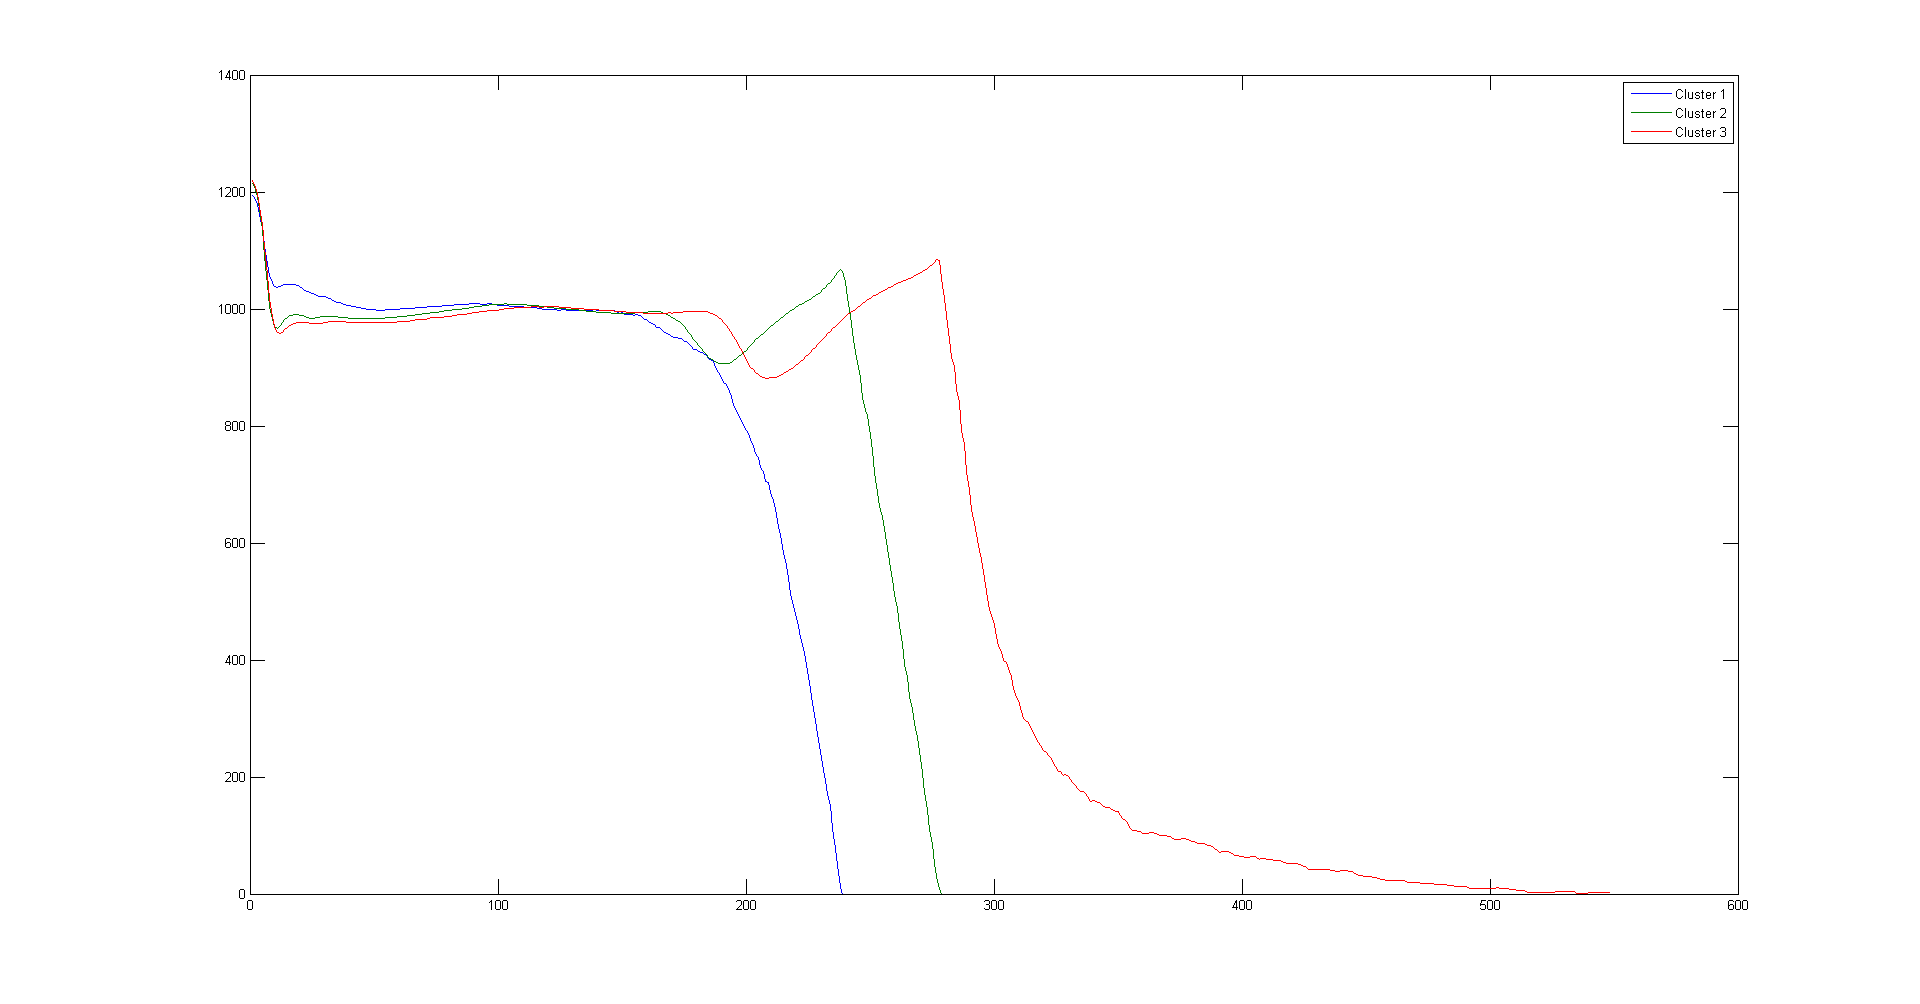
\includegraphics[scale=0.25]{../images/K3Clusters} \\
\begin{lstlisting}   
[I,C] = kmeans(V, 3);   
representatives = zeros(1, 3);
for i = 1:3
    variance = cluster_variance(V(I==i,:), C(i,:));
end

plot(1:size(C,2), C(1,:), 1:size(C,2), C(2,:),1:size(C,2), C(3,:))
\end{lstlisting}

\newpage

	\item[(c)]
		There is no obvious optimal $k$ value. The answer depends on how willing one is to put in additional computational resources in calculating larger values of $k$, if more clusters actually would partition appropriately real life distinct classes, and the variance one is willing to tolerate. One reasonable choice is $k=8$, which is the location on the graph at which the rate of decrease in variance begins to plateau off to a much slower decay.\\
	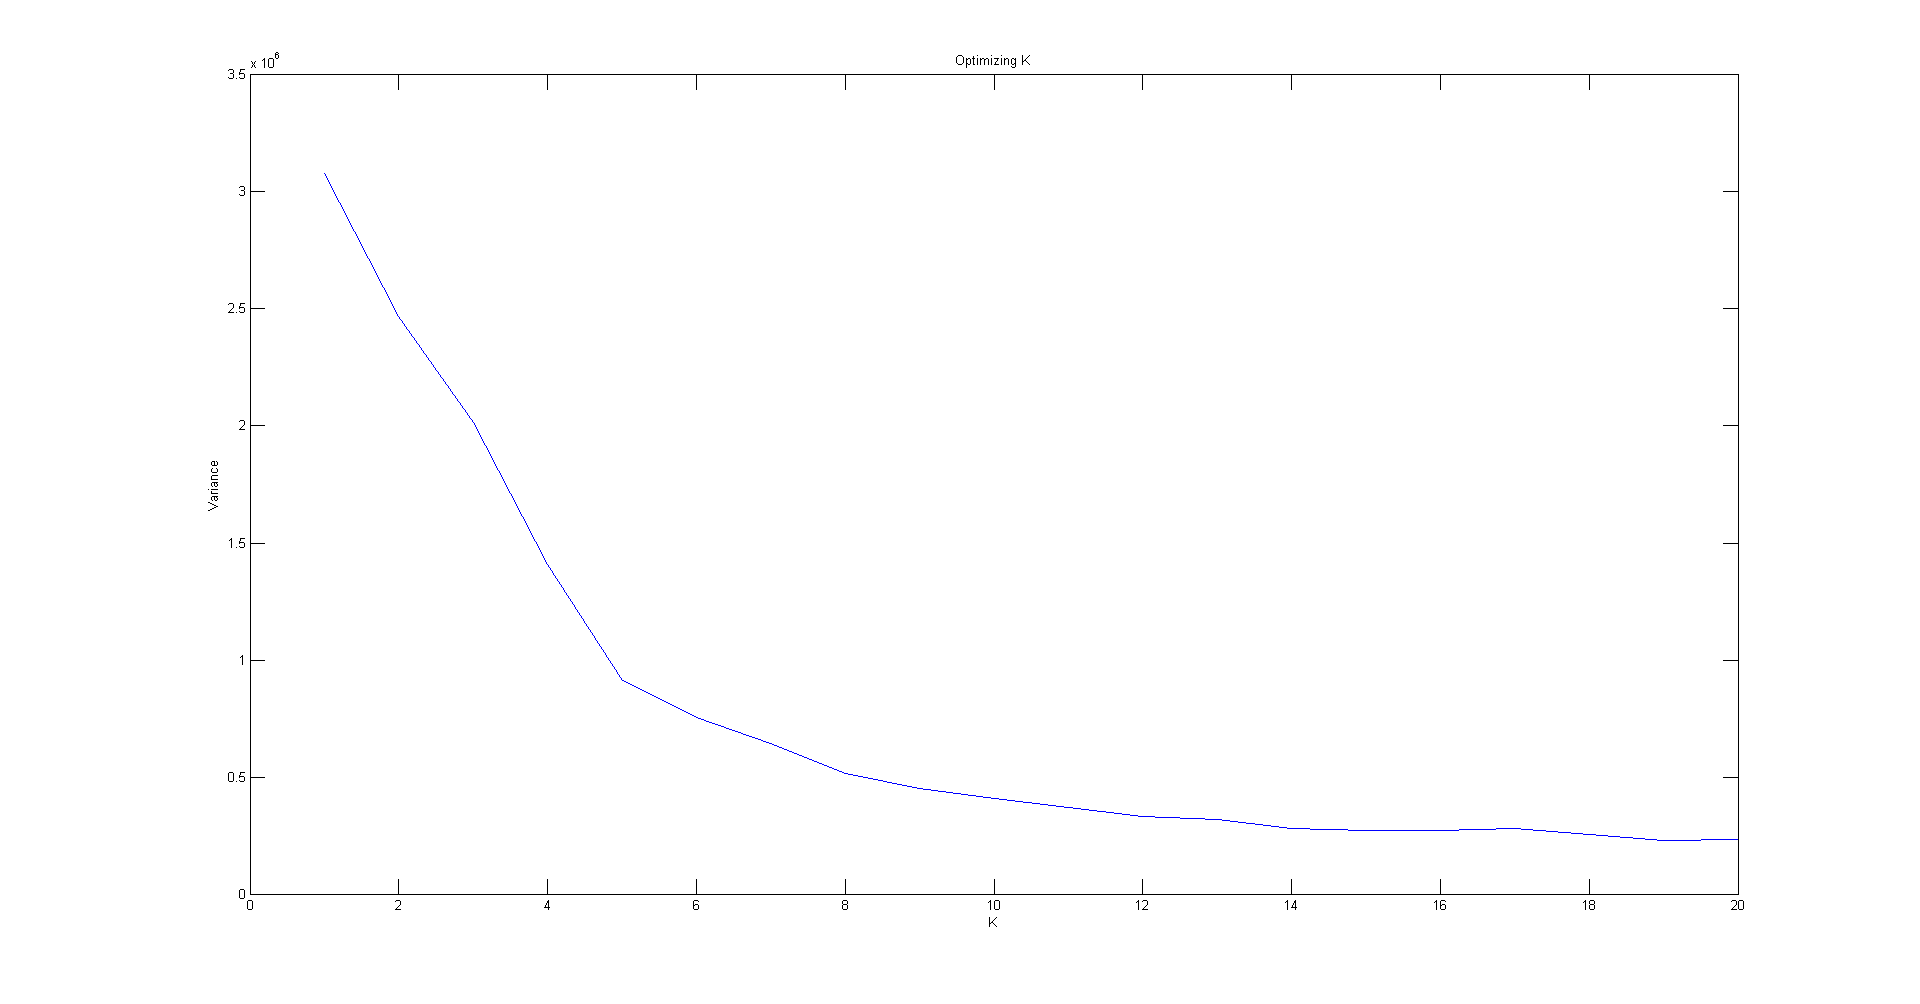
\includegraphics[scale=0.25]{../images/OptimizingK} \\
\begin{lstlisting}   
function [ variance ] = cluster_variance( cluster, centroid )
    points_in_cluster = size(cluster, 1);
    L2 = zeros(1, points_in_cluster);
    for i = 1:points_in_cluster
        L2(i) = norm(cluster(i,:) - centroid);
    end
    variance = var(L2);
end

Ks = 1:20;
variances = zeros(1,length(Ks));
for k = min(Ks):max(Ks)
    [I,C] = kmeans(V, k);   
    cluster_count = size(C, 1);
    variance = zeros(1, cluster_count);
    for i = 1:cluster_count
        variance(i) = cluster_variance(V(I==i,:), C(i,:));
    end
    variances(k) = mean(variance);
end

plot(Ks, variances);
\end{lstlisting}
	\end{enumerate}

\newpage

\item[3.]
	LF/HF ratio: 5.02\\
	This is a normal ratio, so we have no reason to expect that the patient is at risk.\\
\begin{lstlisting}   
function [ XRR1, xrr1 ] = rrfc( xrr0, rrt, fs )
    rrt_linspace = linspace(rrt(1), rrt(end), ((rrt(end)-rrt(1))*fs));
    xrr1 = interp1(rrt, xrr0, rrt_linspace);
    X0 = fft(xrr1);
    XRR1 = fftshift(X0);
end

function [ p ] = signal_power( xrr0, rrt, f1, f2, fs )
    [ XRR1, xrr1] = rrfc( xrr0, rrt, fs);
    N = length(xrr1);
    k1 = N * f1 / fs;
    k2 = N * f2 / fs;
    XRR1s = abs(XRR1).^2;
    p = sum(XRR1s(floor(k1+(N-1)/2):floor(k2+(N-1)/2)))*N;
end

total_time = (23+(52/60)) * 60 * 60;
times = linspace(0, total_time, length(x03));
[pks, locs] = findpeaks(x03, 'MINPEAKHEIGHT', 75);
intervals = diff(times(locs));
rrt = times(locs(2:end));

lf = signal_power(intervals, rrt, 0.04, 0.15, x03_sampling_frequency_in_Hz);
hf = signal_power(intervals, rrt, 0.15, 0.4, x03_sampling_frequency_in_Hz);

ratio = lf/hf
\end{lstlisting}

\end{enumerate}

\end{document}